
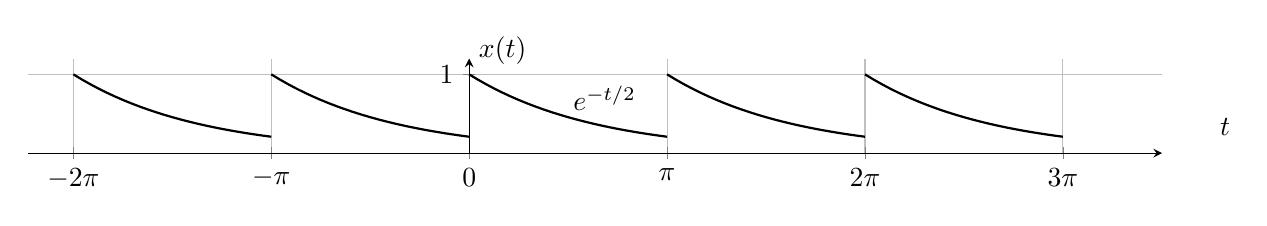
\begin{tikzpicture}
\begin{axis}[grid=both,
	xmin=-7,xmax=11,ymin=0,ymax=1.2,
    y=1cm,
    x=0.8cm,	
    axis y line=middle,
    axis x line=bottom,
    xtick={-6.28319, -3.14159, 0, 3.14159, 6.28319, 9.42478},
    xticklabels={$-2\pi$, $-\pi$, $0$,$\pi$,$2\pi$,$3\pi$},
    ytick={1},
    yticklabels={1},
    xlabel = {$t$},
      ylabel style={
        at={(axis cs:0, 1.3)},
        anchor= west,
    },%
    ylabel = {$x(t)$},
      xlabel style={
        at={(axis cs:12, 0.1)},
        anchor= south,
    },%
    ]
%\addplot[domain=0:pi]  {exp(-x/2)} node[above]{$e^{-t/2}$};
%\addplot [red, domain=pi:2*pi]  {exp(-(x-pi)/2)} node[above]{$e^{-t/2}$};
\foreach \k in { -2,-1,0, 1, 2}
{
	\addplot [thick, domain=\k*pi:	(\k+1)*pi]  {exp(-(x-\k*pi)/2)} ;
}
\node at (axis cs:1.5,0.7) [anchor=west] {$e^{-t/2}$};
\end{axis}
\end{tikzpicture} 